\subsection{External interface Requirements}
The \emph{CLup} frontend is a web application that can be accessed from web browsers. \todo{On modern smartphones, the App will also be installable as a native webapp.} The following section will give a comprehensive description in terms of hardware, software and communication interfaces.

\subsubsection{User interfaces}
\textbf{Login and Registration}\\
When first opening the application, Users are presented with a registration page. They are asked to provide only the essential information: an \emph{e-mail address} and a \emph{password}. The interface also shows a small button to switch to the login page, in case the user has already signed in on another device or the session has expired. The page is identical to the one for the Registration, except for the Login button. In this case, the small button gives the Users the ability to switch back to the registration page, which is needed if multiple people share the same device.
% \begin{figure}[h]
%     \centering
%     \includegraphics[scale=0.63]{Images/login_register2.png}
%     \caption{Registration interface}
% \end{figure}

% \begin{figure}[h]
%     \centering
%     \includegraphics[scale=0.63]{Images/login_register2.png}
%     \caption{Login interface}
% \end{figure}

\textbf{Shop selection page}\\
After login/registration, the app displays a Shop search bar that dynamically updates its results while the Users are typing. After selecting a Shop from the results, the two buttons "Get a Ticket" and "Make a Booking" are enabled, which are linked to the Ticket form and Booking form, respectively.
% \begin{figure}[h]
%     \centering
%     \includegraphics[scale=0.63]{Images/login_register2.png}
%     \caption{Shop search interface}
% \end{figure}

\textbf{Ticket form}\\
This page prompts Users for an optional choice of categories they want to buy. Users can confirm the Ticket request by pressing the "Submit" button. In both the Ticket form and the Booking form, Users are always given option to reset the app back to the Shop selection page.
% \begin{figure}[h]
%     \centering
%     \includegraphics[scale=0.63]{Images/login_register2.png}
%     \caption{Ticket form}
% \end{figure}

\textbf{Booking form}\\
This page is identical to the previous, except for the added time selection. A table with days as columns and hours as rows shows the time slots with lower occupancy. When Users select the preferred day, the visualization updates with specific data for the day, giving an in-depth visualization of restricted to the opening hours. Given this, Users can easily choose a time for their visit. As in the Ticket form, Users can confirm the Booking request by pressing the "Submit" button.
% \begin{figure}[h]
%     \centering
%     \includegraphics[scale=0.63]{Images/login_register2.png}
%     \caption{Booking form}
% \end{figure}

\textbf{Token display}\\
After generating a Ticket or a Booking, and until its expiration, the app will display the token as a fullscreen QR code right after opening, or after Login (if the login timeout has passed).
This makes it very quick to have the Token scanned by the clerks outside of a shop.
% \begin{figure}[h]
%     \centering
%     \includegraphics[scale=0.63]{Images/login_register2.png}
%     \caption{Token display}
% \end{figure}

\subsubsection{Hardware interfaces}
The \emph{CLup} client shall be available for devices capable of rendering a web page with javascript and internet access, this includes smartphones, tablets and personal computers.

Although not strictly required, the devices used by the staff should have a camera to scan QR codes

\subsubsection{Software interfaces}
\begin{itemize}
    \item \textbf{Web browser}: the applicative requires a web browser capable of rendering HTML5 web pages with Javascript
    \item \textbf{Maps service}: although not required for the core functionality, having access to a maps service on the device will improve user experience
\end{itemize}

\subsubsection{Communication interfaces}
\begin{itemize}
    \item \emph{User}: requires a internet connection in order to get a token. Access to the store can be done offline if necessary.
    \item \emph{Staff}: requires a internet connection in order to communicate with the server and validate tokens or emit substitute tickets.
\end{itemize}
The system shall use the HTTPS protocol to provide secure communication from the client to the server.
\subsection{Functional requirements}
\subsubsection{Scenarios}
\textbf{Scenario 1}\\
Maria is gathering ingredients to bake a cake, but she realizes she doesn't have any milk.
Maria lives near to a grocery shop so she opens the web app, she writes the shop name in the search bar and she is presented with the most relevant matches. She clicks on the shop and then she chooses \todo{\emph{"Get a Ticket"}}. Now she checks the dairy section and confirms, receiving her ticket.
CLup shows that Maria's turn will be in about 10 minutes. Five minutes later she checks back on the app and the approximate time is now 5 minutes, so she leaves and she goes to the shop.
At the shop Giovanni, a memeber of the staff, is at the entrance waiting for customers. Maria is welcomed by Giovanni, she opens the application and she shows him the ticket, Giovanni scans the ticket with his phone, Maria is just in time, so she can enter the shop and do her groceries.
At the exit she is invited by Mario, another member of the staff to scan her ticket, she shows the ticket one last time, then she leaves the shop and returns home ready to bake a cake.

\textbf{Scenario 2}\\
Marco has a busy schedule for the week and he needs to go and get a suit for an important meeting. He looks at his schedule and finds a spot on thursday, so he opens the web app, he writes the shop name in the search bar and she is presented with the most relevant matches. He clicks on the shop and then he chooses \todo{\emph{"Book a visit"}}. Then he checks the clothing section and clicks on thursday on the calendar luckily there is a free time slot. So he inputs the time and confirms, the app responds with the token for the booking. On thursday Marco goes to the shop in time for his booking, he is welcomed by Francesca, a staff member, and shows her the QR code associated with his booking, she scans it using her phone and Marco is allowed in. At the exit he is invited to scan his booking one last time before leaving.

\textbf{Scenario 3}\\
Attilio was never a fan of technology and he does not have a smartphone, unfortuanately his grandchild Matteo is not around to get a ticket for him, so he picks up his bicycle and goes to the grocery shop. At the entrance to the shop Francesco, a staff member, informs Attilio about the new procedure to enter the shop, since Attilio does not have a smartphone Fancesco uses his device to create a substitute ticket and prints it. Francesco hands Attilio the ticket, then he tells him that there are already 5 people waiting, so he will have to wait for about 10 minutes. Ten minutes later Attilio goes back to the entrance where Francesco scans the ticket letting Attilio go in. At the exit he is invited to scan the ticket one last time before heading home.

\subsubsection{Use cases}
% Use case name
% Find the actors (concrete names)
% Flow of events with natural language
% Focus on entry and exit condition
% Exceptions

% Use Case Diagrams
\begin{figure}[H]
    \centering
    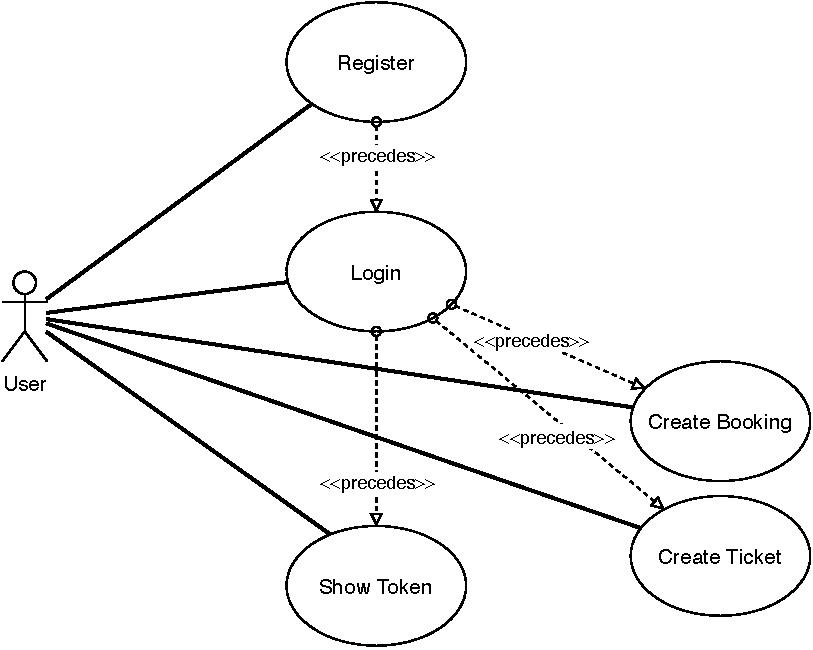
\includegraphics[width=0.7\textwidth]{Images/usecasediagram-user.pdf}
    \caption{Use Case Diagram: User}
\end{figure}
\begin{figure}[H]
    \centering
    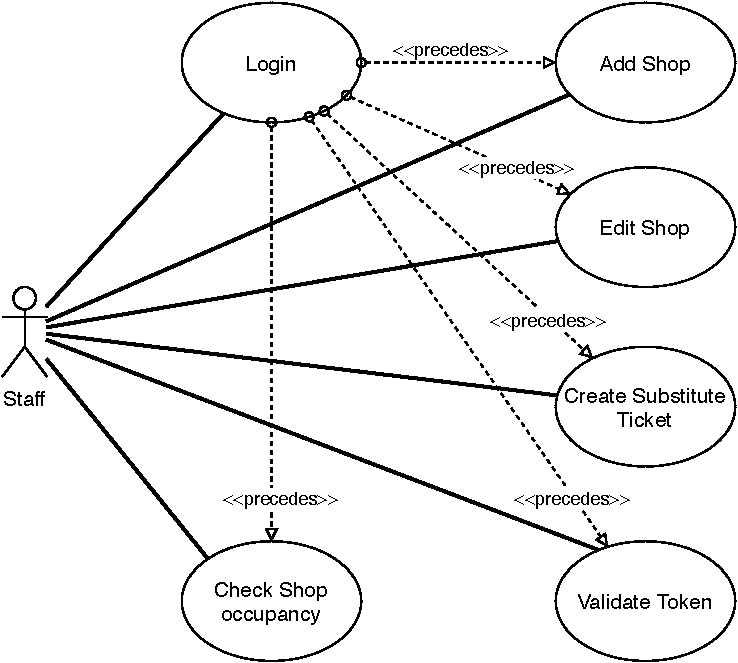
\includegraphics[width=0.7\textwidth]{Images/usecasediagram-staff.pdf}
    \caption{Use Case Diagram: Authority}
\end{figure}

\begin{table}[h]
    \begin{tabularx}{\textwidth}{|X|p{0.75\textwidth}|}
    \hline
    Name           & User creates an account   \\ \hline
    Actor          & Unregistered User \\ \hline
    Entry condition & \begin{itemize}
        \item User has not created an account yet
    \end{itemize}\\ \hline
    Event flow     & \begin{enumerate}
        \item User opens the web app
        \item The app asks for login or registration
        \item The User clicks on register
        \item The User inserts their email and password
        \item The User clicks on confirm
        \item The app prompts the User to check their email for a confirmation linked
        \item The User clicks on the confirmation link
    \end{enumerate} \\ \hline
    \end{tabularx}
\end{table}

\subsubsection{Sequence diagrams}

\subsection{Performance Requirements}
\begin{itemize}
    \item Validating a token must be done as soon as possible and in no more than 5 seconds from when the token was acquired by the staff. This is required to achieve sufficient throughput and prevent queues from forming at the entrance.
    \item When obtaining a token the user shall receive a response from the server within 15 seconds, since in this case time is not critical.
    \item Tokens shall be added to the system as soon as possible within 30 seconds.
\end{itemize}
\subsection{Design constraints}
\subsubsection{Standards compliance}
The web server shall comply to the HTTPS\footnote{\href{https://tools.ietf.org/html/rfc2818}{RFC2818: HTTP Over TLS}} protocol and target the HTTP/2\footnote{\href{https://tools.ietf.org/html/rfc7540}{RFC7540: Hypertext Transfer Protocol Version 2 (HTTP/2)}} standard for communication and the HTML5\footnote{\href{https://www.w3.org/TR/2017/REC-html52-20171214/}{HTML 5.2 W3C Recommendation, 14 December 2017}} standard for web pages.

\subsubsection{Hardware limitations}
Running the app requires a smartphone that supports one of the modern web browser engines; older cellphones whose official support has been discontinued shall not be supported.
To allow the validation of tickets by the Third Party Staff, the device should also be equipped with a camera of any resolution above 8 Megapixel.
%\subsubsection{Other constraints}

\subsection{Software System Attributes}
\subsubsection{Reliability}
\textit{CLup} should be available 24/7 in order to allow Users to generate Tokens at any time of the day. Downtime due to maintenance shall be during the night and no longer than 2 hours, furthermore, users and third parties shall be notified at least 3 days prior the scheduled downtime.
\subsubsection{Availability}
\emph{CLup} does not have a critical nature, however any downtime could cause serious problems to the management of the entrances to Shops. Hence, 99\% availability during daytime is required for \emph{CLup} to be effective. At night time, the availability requirement can be relaxed to 95\%.
\subsubsection{Security}
All communication should be over HTTPS protocol to provide privacy, data integrity and authentication.
User passwords shall be stored in a salted hash format.
The system should keep thorough logs of the activity of logged in users and of login attempts. The registration and login procedure should not disclose informations about existing users and repeated login attempts shall be limited.
Further details about the cryptographic functions and protocols employed will be discussed in the Design Document.
\subsubsection{Maintainability}
The system components shall be realized with high modularity and orthogonality between modules. This allows modifications to the code to be localized and leave the other components unaffected, minimizing the time required to fix problems with the system.
The backend system shall be able to run a test instance of the service that can be used by developers to test out features before deploying them to the main instance.
\subsubsection{Portability}
\textit{Clup} should be easily deployable on a dedicated machine, on a virtual private server or on a cloud hosting service. The server should be able to run both natively and in a containerized environment for maximum portability.
